% pipeline_diagram.tex  —  PPO training loop bottlenecks and JAX optimisations
% Compile: pdflatex pipeline_diagram.tex

\documentclass[tikz, border=14pt]{standalone}
\usepackage{tikz}
\usepackage{amsmath}
\usepackage[T1]{fontenc}
\usepackage{lmodern}
\usetikzlibrary{
  arrows.meta, shapes.geometric, positioning,
  fit, backgrounds, decorations.pathreplacing, calc
}

%% ── Colours ─────────────────────────────────────────────────────────────────
\definecolor{navy}      {RGB}{ 28,  48,  88}
\definecolor{navymed}   {RGB}{ 58,  90, 150}
\definecolor{stagefill} {RGB}{245, 247, 252}
\definecolor{t2red}     {RGB}{198,  52,  42}
\definecolor{t2bg}      {RGB}{252, 235, 232}
\definecolor{t4green}   {RGB}{ 34, 139,  80}
\definecolor{t4bg}      {RGB}{225, 248, 232}
\definecolor{badgecol}  {RGB}{210, 110,   5}
\definecolor{badgebg}   {RGB}{255, 248, 215}
\definecolor{summbg}    {RGB}{230, 242, 255}
\definecolor{graydash}  {RGB}{150, 165, 185}

%% ── Column geometry ─────────────────────────────────────────────────────────
\def\colA{-82.5mm}
\def\colB{-27.5mm}
\def\colC{ 27.5mm}
\def\colD{ 82.5mm}
\def\colW{44mm}
\def\codeW{41mm}

%% ── Row y-positions ─────────────────────────────────────────────────────────
%  In TikZ y increases upward, so more negative = lower on page.
%  T2 boxes: anchor=north at \yTtwo  (~28 mm tall → bottom ≈ \yTtwo − 28mm)
%  Badges sit between T2 bottom and T4 top.
%  T4 boxes: anchor=north at \yTfour (~30 mm tall → bottom ≈ \yTfour − 30mm)
\def\yHeader  {  0mm}
\def\yStage   {-20mm}
\def\yTtwo    {-42mm}   % TOP of Tier-2 code boxes
\def\yBadge   {-76mm}   % speed badges  (≈ 6 mm above T4 tops)
\def\yTfour   {-82mm}   % TOP of Tier-4 code boxes
\def\ySummary {-122mm}
\def\yLegend  {-136mm}

%% ── Shared styles ────────────────────────────────────────────────────────────
\tikzset{
  stagebox/.style={
    rectangle, rounded corners=5pt,
    minimum width=\colW, minimum height=14mm,
    fill=stagefill, draw=navymed, line width=0.85pt,
    align=center, font=\small\bfseries\sffamily, text=navy
  },
  t2box/.style={
    rectangle, rounded corners=3pt,
    minimum width=\codeW, text width=\codeW,
    inner xsep=5pt, inner ysep=6pt,
    fill=t2bg, draw=t2red!55, line width=0.55pt,
    align=left,
    font=\fontsize{6.8}{9}\selectfont\ttfamily
  },
  t4box/.style={
    rectangle, rounded corners=3pt,
    minimum width=\codeW, text width=\codeW,
    inner xsep=5pt, inner ysep=6pt,
    fill=t4bg, draw=t4green!55, line width=0.55pt,
    align=left,
    font=\fontsize{6.8}{9}\selectfont\ttfamily
  },
  badge/.style={
    rectangle, rounded corners=7pt,
    fill=badgebg, draw=badgecol, line width=0.65pt,
    inner xsep=5pt, inner ysep=2.5pt,
    font=\fontsize{8}{9.5}\selectfont\bfseries\sffamily,
    text=badgecol
  },
  pipeArrow/.style={
    ->, >={Stealth[length=7pt,width=5pt]},
    line width=1.7pt, color=navymed
  },
}

\begin{document}
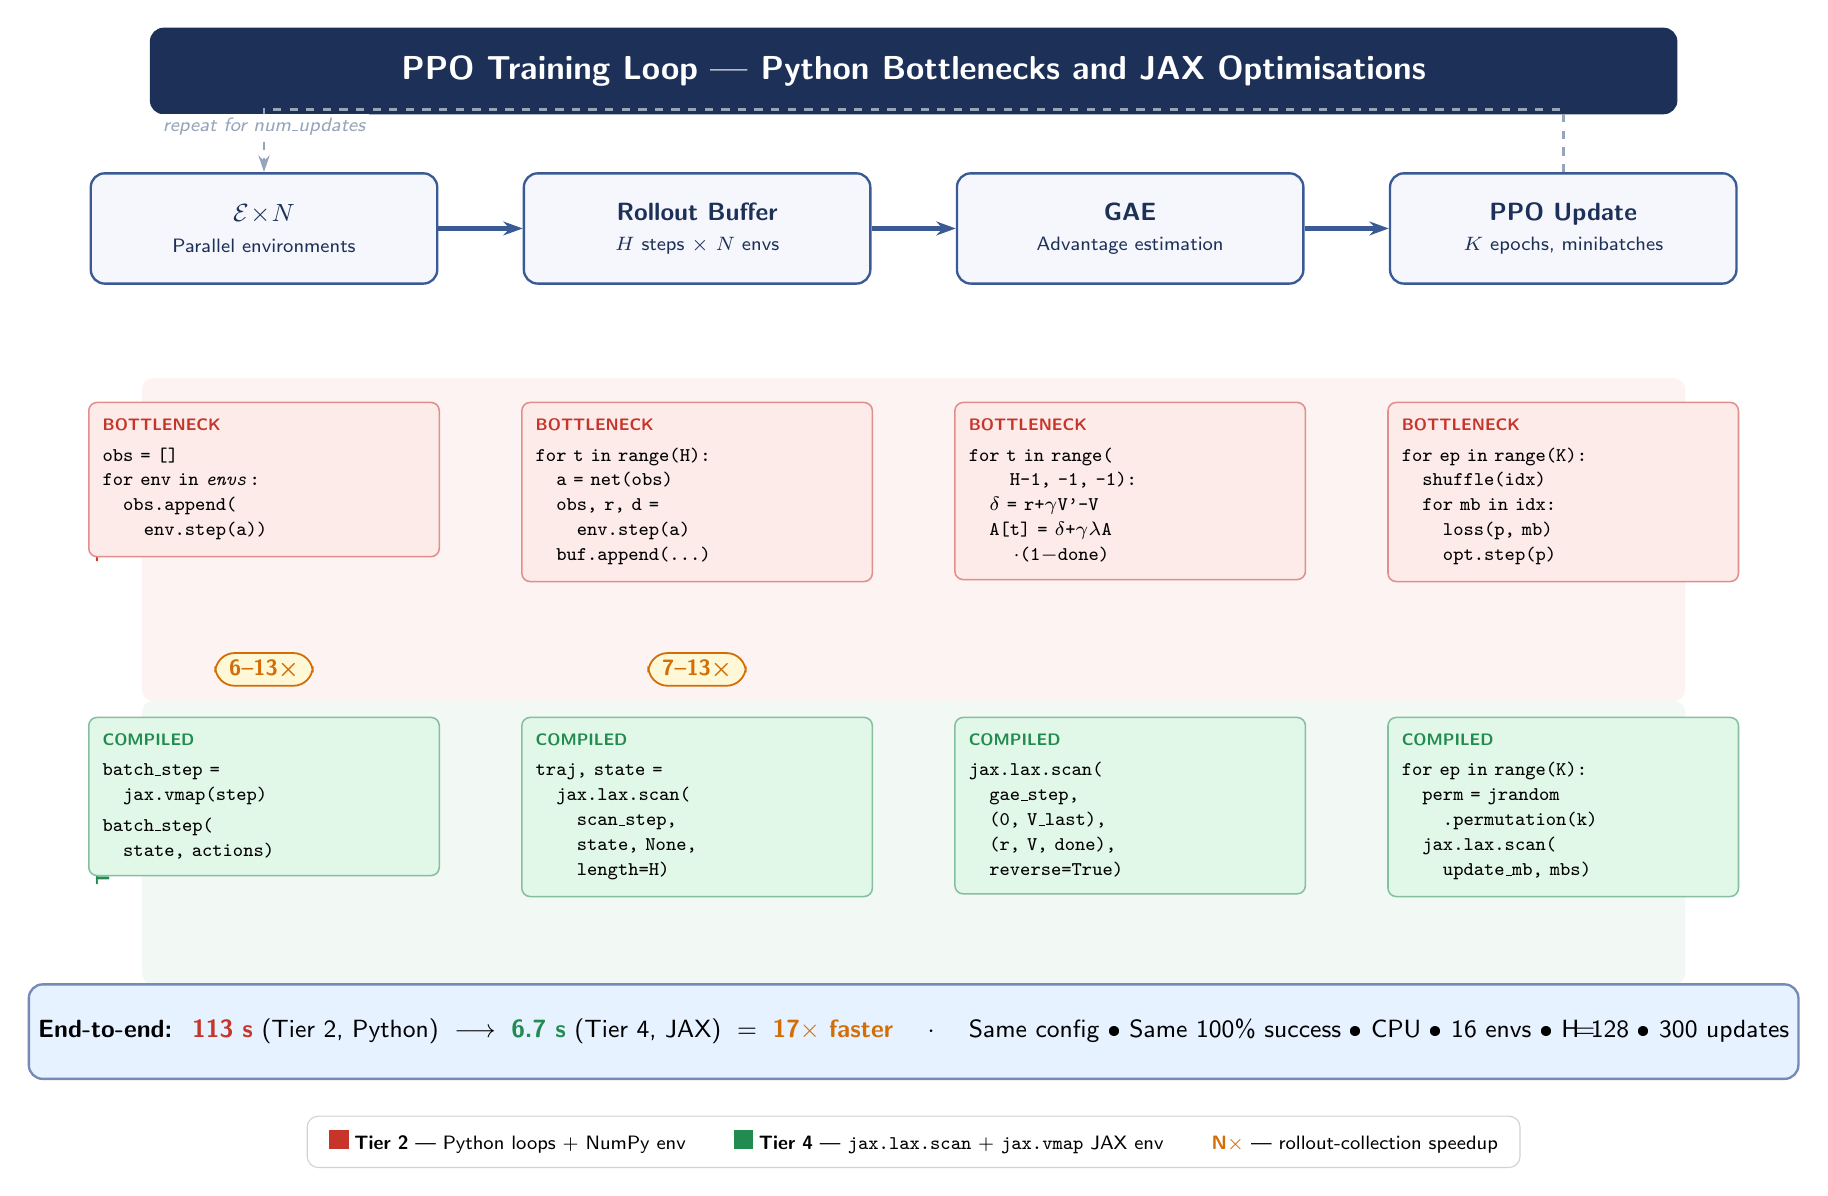
\begin{tikzpicture}

%% ════════════════════════════════════════════════════════════════════════════
%%  HEADER
%% ════════════════════════════════════════════════════════════════════════════
\node[
  rectangle, rounded corners=5pt,
  fill=navy, text=white,
  minimum width=194mm, minimum height=11mm,
  align=center, font=\large\bfseries\sffamily
] (header) at (0,\yHeader)
  {PPO Training Loop \textrm{—} Python Bottlenecks and JAX Optimisations};

%% ════════════════════════════════════════════════════════════════════════════
%%  ROW LABELS  (x = −103 mm, well clear of column A at −82.5 mm)
%% ════════════════════════════════════════════════════════════════════════════
\node[rotate=90, font=\fontsize{7.5}{9}\selectfont\bfseries\sffamily, text=navy]
  at (-103mm, \yStage) {Stage};

% Tier-2 label centred vertically in its band: midpoint of −42 mm to −76 mm = −59 mm
\node[rotate=90, font=\fontsize{7.5}{9}\selectfont\bfseries\sffamily, text=t2red]
  at (-103mm, -59mm) {Tier 2};

% Tier-4 label centred vertically in its band: midpoint of −82 mm to −118 mm = −100 mm
\node[rotate=90, font=\fontsize{7.5}{9}\selectfont\bfseries\sffamily, text=t4green]
  at (-103mm, -100mm) {Tier 4};

%% ════════════════════════════════════════════════════════════════════════════
%%  STAGE BOXES
%% ════════════════════════════════════════════════════════════════════════════
\node[stagebox] (s1) at (\colA, \yStage)
  {$\mathcal{E}\!\times\!N$\\\normalfont\scriptsize\sffamily Parallel environments};

\node[stagebox] (s2) at (\colB, \yStage)
  {Rollout Buffer\\\normalfont\scriptsize\sffamily $H$ steps $\times$ $N$ envs};

\node[stagebox] (s3) at (\colC, \yStage)
  {GAE\\\normalfont\scriptsize\sffamily Advantage estimation};

\node[stagebox] (s4) at (\colD, \yStage)
  {PPO Update\\\normalfont\scriptsize\sffamily $K$ epochs, minibatches};

%% ── Pipeline arrows ─────────────────────────────────────────────────────────
\draw[pipeArrow] (s1.east) -- (s2.west);
\draw[pipeArrow] (s2.east) -- (s3.west);
\draw[pipeArrow] (s3.east) -- (s4.west);

%% ── Feedback arrow ──────────────────────────────────────────────────────────
\draw[->, >={Stealth[length=6pt,width=4pt]}, line width=1pt, dashed, color=graydash]
  (s4.north) -- ++(0,8mm)
  -- ++(-165mm,0)
  -- (s1.north)
  node[pos=0.5, above, font=\fontsize{7}{8.5}\selectfont\sffamily\itshape,
       text=graydash, fill=white, inner sep=1.5pt]
  {repeat for \textit{num\_updates}};

%% ════════════════════════════════════════════════════════════════════════════
%%  TIER-2 CODE BOXES  (anchor = north → top edge at \yTtwo)
%% ════════════════════════════════════════════════════════════════════════════
\node[t2box, anchor=north] (t2a) at (\colA, \yTtwo) {%
  {\color{t2red}\fontsize{6.2}{7.5}\selectfont\bfseries\sffamily BOTTLENECK}\\[2pt]%
  obs = []\\
  for env in \textit{envs}:\\
  \quad obs.append(\\
  \quad\quad env.step(a))%
};

\node[t2box, anchor=north] (t2b) at (\colB, \yTtwo) {%
  {\color{t2red}\fontsize{6.2}{7.5}\selectfont\bfseries\sffamily BOTTLENECK}\\[2pt]%
  for t in range(H):\\
  \quad a = net(obs)\\
  \quad obs, r, d =\\
  \quad\quad env.step(a)\\
  \quad buf.append(...)%
};

\node[t2box, anchor=north] (t2c) at (\colC, \yTtwo) {%
  {\color{t2red}\fontsize{6.2}{7.5}\selectfont\bfseries\sffamily BOTTLENECK}\\[2pt]%
  for t in range(\\
  \quad\quad H-1, -1, -1):\\
  \quad $\delta$ = r+$\gamma$V'-V\\
  \quad A[t] = $\delta$+$\gamma\lambda$A\\
  \quad\quad\,$\cdot$(1$-$done)%
};

\node[t2box, anchor=north] (t2d) at (\colD, \yTtwo) {%
  {\color{t2red}\fontsize{6.2}{7.5}\selectfont\bfseries\sffamily BOTTLENECK}\\[2pt]%
  for ep in range(K):\\
  \quad shuffle(idx)\\
  \quad for mb in idx:\\
  \quad\quad loss(p, mb)\\
  \quad\quad opt.step(p)%
};

%% ── Speed badges (centred between T2 bottoms and T4 tops) ───────────────────
\node[badge] at (\colA, \yBadge) {\textbf{6–13}$\boldsymbol{\times}$};
\node[badge] at (\colB, \yBadge) {\textbf{7–13}$\boldsymbol{\times}$};

%% ════════════════════════════════════════════════════════════════════════════
%%  TIER-4 CODE BOXES  (anchor = north → top edge at \yTfour)
%% ════════════════════════════════════════════════════════════════════════════
\node[t4box, anchor=north] (t4a) at (\colA, \yTfour) {%
  {\color{t4green}\fontsize{6.2}{7.5}\selectfont\bfseries\sffamily COMPILED}\\[2pt]%
  batch\_step =\\
  \quad jax.vmap(step)\\[2pt]%
  batch\_step(\\
  \quad state, actions)%
};

\node[t4box, anchor=north] (t4b) at (\colB, \yTfour) {%
  {\color{t4green}\fontsize{6.2}{7.5}\selectfont\bfseries\sffamily COMPILED}\\[2pt]%
  traj, state =\\
  \quad jax.lax.scan(\\
  \quad\quad scan\_step,\\
  \quad\quad state, None,\\
  \quad\quad length=H)%
};

\node[t4box, anchor=north] (t4c) at (\colC, \yTfour) {%
  {\color{t4green}\fontsize{6.2}{7.5}\selectfont\bfseries\sffamily COMPILED}\\[2pt]%
  jax.lax.scan(\\
  \quad gae\_step,\\
  \quad (0, V\_last),\\
  \quad (r, V, done),\\
  \quad reverse=True)%
};

\node[t4box, anchor=north] (t4d) at (\colD, \yTfour) {%
  {\color{t4green}\fontsize{6.2}{7.5}\selectfont\bfseries\sffamily COMPILED}\\[2pt]%
  for ep in range(K):\\
  \quad perm = jrandom\\
  \quad\quad .permutation(k)\\
  \quad jax.lax.scan(\\
  \quad\quad update\_mb, mbs)%
};

%% ════════════════════════════════════════════════════════════════════════════
%%  BACKGROUND BANDS
%% ════════════════════════════════════════════════════════════════════════════
\begin{scope}[on background layer]
  % Tier-2 band: from just above T2 tops to midpoint between rows
  \fill[t2red!6, rounded corners=4pt]
    (-98mm, \yTtwo + 3mm) rectangle (98mm, \yBadge - 4mm);
  % Tier-4 band: from midpoint to just below summary
  \fill[t4green!6, rounded corners=4pt]
    (-98mm, \yBadge - 4mm) rectangle (98mm, \ySummary + 6mm);
\end{scope}

%% ════════════════════════════════════════════════════════════════════════════
%%  SUMMARY BAR
%% ════════════════════════════════════════════════════════════════════════════
\node[
  rectangle, rounded corners=5pt,
  fill=summbg, draw=navymed!70, line width=0.85pt,
  minimum width=194mm, minimum height=12mm,
  align=center, font=\small\sffamily
] at (0, \ySummary)
  {\textbf{End-to-end:} \
   \textcolor{t2red}{\textbf{113 s}} (Tier 2, Python)
   $\;\longrightarrow\;$
   \textcolor{t4green}{\textbf{6.7 s}} (Tier 4, JAX)
   $\;=\;$
   \textcolor{badgecol}{\textbf{17$\times$ faster}}
   $\quad\cdot\quad$
   \textsf{Same config~\textbullet~Same 100\% success~\textbullet~CPU~\textbullet~16 envs~\textbullet~H\!=\!128~\textbullet~300 updates}};

%% ════════════════════════════════════════════════════════════════════════════
%%  LEGEND
%% ════════════════════════════════════════════════════════════════════════════
\node[
  rectangle, rounded corners=4pt,
  draw=gray!35, fill=white,
  inner xsep=8pt, inner ysep=5pt,
  font=\fontsize{7.5}{9.5}\selectfont\sffamily, align=center
] at (0, \yLegend)
  {\textcolor{t2red}{\rule{7pt}{7pt}}\;%
   \textbf{Tier 2}~—~Python loops + NumPy env
   \qquad
   \textcolor{t4green}{\rule{7pt}{7pt}}\;%
   \textbf{Tier 4}~—~\texttt{jax.lax.scan} + \texttt{jax.vmap} JAX env
   \qquad
   \textcolor{badgecol}{\textbf{N$\times$}}~—~rollout-collection speedup};

\end{tikzpicture}
\end{document}
